%%%%%%%%%%%%%%%%%%%%%%%%%%%%%%%%%%%%%%%%%%%%%%%
%
% Template per Elaborato di Laurea
% DISI - Dipartimento di Ingegneria e Scienza dell’Informazione
%
% update 2015-09-10
%
% Per la generazione corretta del
% pdflatex nome_file.tex
% bibtex nome_file.aux
% pdflatex nome_file.tex
% pdflatex nome_file.tex
%
%%%%%%%%%%%%%%%%%%%%%%%%%%%%%%%%%%%%%%%%%%%%%%%

% formato FRONTE RETRO
\IfFileExists{./.draft}{
  \documentclass[epsfig,a4paper,11pt,titlepage,twoside,openany,draft]{book}
}{
  \documentclass[epsfig,a4paper,11pt,titlepage,twoside,openany]{book}
}

\usepackage{epsfig}
\usepackage{plain}
\usepackage{setspace}
\usepackage[paperheight=29.7cm,paperwidth=21cm,outer=1.5cm,inner=2.5cm,top=2cm,bottom=2cm]{geometry} % per definizione layout
\usepackage{titlesec} % per formato custom dei titoli dei capitoli
\usepackage[utf8x]{inputenc} % per Linux (richiede il pacchetto unicode);

\usepackage{acronym}
\usepackage{mdwlist}
\usepackage{easy-todo}
\usepackage{minted}
\usepackage{booktabs}

\usepackage{hyperref} % this should be the last imported

\acrodef{IPA}{International Publishers Association}
\acrodef{STM}{International Association of Scientific, Technical and Medical Publishers}
\acrodef{AAP}{Association of American Publishers}

\acrodef{MAG}{Microsoft Academic Graph}
\acrodef{CCDF}{Complementary Cumulative Distribution Function}

\acrodef{SBN}{Standard Book Numbering}
\acrodef{ISO}{International Organization for Standardization}
\acrodef{DOI}{Document Object Identifier}
\acrodef{ISBN}{International Standard Book Number}
\acrodef{PMID}{PubMed Unique Identifier}

\acrodef{RDD}{Resilient Distributed Dataset}
\acrodef{CSV}{Comma-separated Values}

\singlespacing{}

\usepackage[english]{babel}

\begin{document}

  % nessuna numerazione
  \pagenumbering{gobble}
  % !TEX root = thesis.tex

\pagestyle{plain}

\thispagestyle{empty}

\begin{center}
  \begin{figure}[h!]
    \centerline{\psfig{file=logo_unitn_black_center.eps,width=0.6\textwidth}}
  \end{figure}

  \vspace{2 cm}

  \LARGE{Department of Information Engineering and Computer Science\\}
  % \LARGE{Dipartimento di Ingegneria e Scienza dell’Informazione\\}

  \vspace{1 cm}
  \Large{Master Degree in Computer Science\\
    %Informatica
    %Ingegneria dell'Informazione e delle Comunicazioni
    %Ingegneria dell'Informazione e Organizzazione d'Impresa
    %Ingegneria Elettronica e delle Telecomunicazioni
  }

  \vspace{2 cm}
  \Large\textsc{Final Thesis\\}
  \vspace{1 cm}
  \Huge\textsc{An analysis of scholarly citations in Wikipedia\\}
  % \Large{\it{TODO: Sottotitolo (alcune volte lungo - opzionale)}}


  \vspace{2 cm}
  \begin{tabular*}{\textwidth}{ c @{\extracolsep{\fill}} c }
  \Large{Supervisor} & \Large{Graduand}\\
  \Large{Prof.\ Alberto Montresor}& \Large{Alessio Bogon}\\
  \Large{Co-Supervisor} & \\
  \Large{Cristian Consonni} & \\
  \end{tabular*}

  \vspace{2 cm}

  \Large{Academic year 2014/2015}

\end{center}


  \clearpage

%%%%%%%%%%%%%%%%%%%%%%%%%%%%%%%%%%%%%%%%%%%%%%%%%%%%%%%%%%%%%%%%%%%%%%%%%%
%%%%%%%%%%%%%%%%%%%%%%%%%%%%%%%%%%%%%%%%%%%%%%%%%%%%%%%%%%%%%%%%%%%%%%%%%%
%% Nota
%%%%%%%%%%%%%%%%%%%%%%%%%%%%%%%%%%%%%%%%%%%%%%%%%%%%%%%%%%%%%%%%%%%%%%%%%%
%% Sezione Ringraziamenti opzionale
%%%%%%%%%%%%%%%%%%%%%%%%%%%%%%%%%%%%%%%%%%%%%%%%%%%%%%%%%%%%%%%%%%%%%%%%%%
%%%%%%%%%%%%%%%%%%%%%%%%%%%%%%%%%%%%%%%%%%%%%%%%%%%%%%%%%%%%%%%%%%%%%%%%%%
  % !TEX root = thesis.tex

\thispagestyle{empty}

\begin{center}
  {\bf \Huge  \emph{Acknowledgements}}
\end{center}
\vspace{4cm}
{\em \centering
My gratitude goes to my parents and my grandparents,

which always support all my choices and always believe in me.

I want to thank my mum, which is always present and ready to console me whenever I need.

A heartfelt thanks goes to all of my friends that could bear me up to this point,

especially to Davide which shared with me the long journey that started ten years ago.

}

  \clearpage
  \pagestyle{plain} % nessuna intestazione e pie pagina con numero al centro


  % inizio numerazione pagine in numeri arabi
  \mainmatter{}

%%%%%%%%%%%%%%%%%%%%%%%%%%%%%%%%%%%%%%%%%%%%%%%%%%%%%%%%%%%%%%%%%%%%%%%%%%
%%%%%%%%%%%%%%%%%%%%%%%%%%%%%%%%%%%%%%%%%%%%%%%%%%%%%%%%%%%%%%%%%%%%%%%%%%
%% Nota
%%%%%%%%%%%%%%%%%%%%%%%%%%%%%%%%%%%%%%%%%%%%%%%%%%%%%%%%%%%%%%%%%%%%%%%%%%
%% Si ricorda che il numero massimo di facciate e' 30.
%% Nel conteggio delle facciate sono incluse
%%   indice
%%   sommario
%%   capitoli
%% Dal conteggio delle facciate sono escluse
%%   frontespizio
%%   ringraziamenti
%%   allegati
%%%%%%%%%%%%%%%%%%%%%%%%%%%%%%%%%%%%%%%%%%%%%%%%%%%%%%%%%%%%%%%%%%%%%%%%%%
%%%%%%%%%%%%%%%%%%%%%%%%%%%%%%%%%%%%%%%%%%%%%%%%%%%%%%%%%%%%%%%%%%%%%%%%%%

    % indice
    \tableofcontents
    \clearpage



    % gruppo per definizone di successione capitoli senza interruzione di pagina
    \begingroup
      % nessuna interruzione di pagina tra capitoli
      % ridefinizione dei comandi di clear page
      \renewcommand{\cleardoublepage}{}
      \renewcommand{\clearpage}{}
      % redefinizione del formato del titolo del capitolo
      % da formato
      %   Capitolo X
      %   Titolo capitolo
      % a formato
      %   X   Titolo capitolo

      \titleformat{\chapter}
        {\normalfont\Huge\bfseries}{\thechapter}{1em}{}

      \titlespacing*{\chapter}{0pt}{0.59in}{0.02in}
      \titlespacing*{\section}{0pt}{0.20in}{0.02in}
      \titlespacing*{\subsection}{0pt}{0.10in}{0.02in}

      % sommario
      % !TEX root = thesis.tex

\chapter*{Introduction} % without page enumeration
\label{introduction}
\addcontentsline{toc}{chapter}{Introduction} % add me to the index anyway
\todo{Purpose of this study? What do we want to achieve? What should we do next?}

Sommario è un breve riassunto del lavoro svolto dove si descrive l'obiettivo, l'oggetto della tesi, le
metodologie e le tecniche usate, i dati elaborati e la spiegazione delle conclusioni alle quali siete arrivati.

Il sommario dell’elaborato consiste al massimo di 3 pagine e deve contenere le seguenti informazioni:
\begin{itemize}
  \item contesto e motivazioni
  \item breve riassunto del problema affrontato
  \item tecniche utilizzate e/o sviluppate
  \item risultati raggiunti, sottolineando il contributo personale del laureando/a
\end{itemize}

%%%%%%%%%%%%%%%%%%%%%%%%%%%%%%%%%%%%%%%%%%%%%%%%%%%%%%%%%%%%%%%%%%%%%%%%%%
%%%%%%%%%%%%%%%%%%%%%%%%%%%%%%%%%%%%%%%%%%%%%%%%%%%%%%%%%%%%%%%%%%%%%%%%%%
%% Nota
%%%%%%%%%%%%%%%%%%%%%%%%%%%%%%%%%%%%%%%%%%%%%%%%%%%%%%%%%%%%%%%%%%%%%%%%%%
%% Sommario e' un breve riassunto del lavoro svolto dove si descrive
%% l’obiettivo, l’oggetto della tesi, le metodologie e
%% le tecniche usate, i dati elaborati e la spiegazione delle conclusioni
%% alle quali siete arrivati.
%% Il sommario dell’elaborato consiste al massimo di 3 pagine e deve contenere le seguenti informazioni:
%%   contesto e motivazioni
%%   breve riassunto del problema affrontato
%%   tecniche utilizzate e/o sviluppate
%%   risultati raggiunti, sottolineando il contributo personale del laureando/a
%%%%%%%%%%%%%%%%%%%%%%%%%%%%%%%%%%%%%%%%%%%%%%%%%%%%%%%%%%%%%%%%%%%%%%%%%%
%%%%%%%%%%%%%%%%%%%%%%%%%%%%%%%%%%%%%%%%%%%%%%%%%%%%%%%%%%%%%%%%%%%%%%%%%%

      %%%%%%%%%%%%%%%%%%%%%%%%%%%%%%%%
      % lista dei capitoli
      %
      % \input oppure \include
      %
      \newpage
      % !TEX root = thesis.tex

\chapter{Background and related work}
\label{cha:background}
TODO


\section{Wikipedia}
\label{sec:wiki}
Wikipedia is a free-access, free-content Internet encyclopedia, supported and hosted by the non-profit Wikimedia Foundation.
Contributors can access the site can edit most of its articles.
Wikipedia is ranked among the ten most popular websites, and constitutes the Internet's largest and most popular general reference work.
%TODO: CITEME: Bill Tancer (May 1, 2007). "Look Who's Using Wikipedia". Time. Retrieved December 1, 2007. The sheer volume of content [...] is partly responsible for the site's dominance as an online reference. When compared to the top 3,200 educational reference sites in the US, Wikipedia is No. 1, capturing 24.3% of all visits to the category. Cf. Bill Tancer (Global Manager, Hitwise), "Wikipedia, Search and School Homework", Hitwise, March 1, 2007.

\subsection{Structure}
\label{ssec:wiki_structure}
In this section we describe the various entities that compose Wikipedia which are relevant to our analysis.

The basic block of Wikipedia is the \emph{page}.
Pages are plain text document that can be customized using the wiki markup language, which is rendered when a user requests it.
A Wikipedia \emph{article}, or entry, is a page that has encyclopedic information on it.
A well-written encyclopedia article identifies a notable encyclopedic topic, summarizes that topic comprehensively, contains references to reliable sources, and links to other related topics.

A Wikipedia \emph{namespace} is a set of Wikipedia pages whose names begin with a particular reserved word recognized by the MediaWiki software (followed by a colon).
For example, in the user namespace all titles begin with ``User:''.
In the case of the article (or main) namespace, in which encyclopedia articles appear, the reserved word and colon are absent.

At the time of writing, Wikipedia has 35 current namespaces: 16 subject namespaces, 16 corresponding talk namespaces, 2 virtual namespaces, and 1 special namespace.

Pages under the virtual namespaces (``Special'' and ``Media'') are not actually stored in the wikipedia database.
Special pages are created on demand by the MediaWiki software: for instance, ``Special:Log'' lists the log of all the activities on Wikipedia.
Files like images, videos and other assets live under the ``Media'' namespace.

Every time a contributor edits a page, a new \emph{revision} is created.
It contains the text of the new version, as well as information about the contributor, the timestamp, the comment and others.

\section{Microsoft Academic Service}
\label{sec:mag}
Microsoft Academic Search is an experimental research service developed by Microsoft Research to explore how scholars, scientists, students, and practitioners find academic content, researchers, institutions, and activities.
According to the authors, the service has already indexed 83 million papers achieving an above-95\% accuracy~\cite{Sinha2015}.
The service can also display the key relationships between and among subjects, content, and authors, highlighting the critical links that help define scientific research.

For these reasons, we use this service in our analysis.
The dataset is available under the name of ``Microsoft Academic Graph''.

The available entities relevant to our research are the following:
\begin{description*}
    \item[Papers] Contains information like the name of the paper, the publication date, its \ac{DOI} (if available), the journal or the conference where it appeared on.
    \item[PaperReferences] Contains the references between papers.
    \item[Journals] Contains the list of journals.
    \item[Conference] Contains the list of conferences.
\end{description*}



\section{Related work}
\label{sec:relatedwork}

      \newpage
      % !TEX root = thesis.tex

\chapter{System architecture}
\label{cha:system_architecture}
This section analyzes in detail the structure of the datasets, their problems and their peculiarities.
Also, we give a description of the machines used to execute our software, together with a description of what the various components do.

\section{Infrastructure}
\label{sec:infrastructure}
The various software components have been written and tested on a MacBook Pro.
Its specification can be found in Table~\ref{tbl:tech_specs}.
Its storage is limited to 500 GB and because of the size of our datasets it was not possible to run the programs on all of them.

For this reason University of Trento allowed us to use one of their machines called ``adige''.
Its hardware is not very different from the MacBook (see Table~\ref{tbl:tech_specs}).
Since we are going to need at least 866 GB just to store the Wikimedia page view statistics, the network office also allocated a 4 TB network disk.
This machine is always on, so we can launch the programs and retrieve the results as soon as they finish, without worrying of system reboots.

Even though the disk space is not a problem, the processing power is still an issue when we want to sort the page view statistics, as described in Sect.~\ref{sub:Sorting pagecounts}.
To mitigate this problem, we exploit the UniTN Cisca cluster.
It consist of circa 125 workstations, each of them having 4 cores available.
The technical specifications of the single workstation are not impressive (see Table~\ref{tbl:tech_specs}), but the fact that we can use more than 500 cores in total makes the difference.
\todo{explain the difficulty with working with torque}

\begin{table}[]
\centering
\caption{Technical specification of the machines used.}
\label{tbl:tech_specs}
\begin{tabular}{@{}lrrr@{}}
\toprule
\multicolumn{1}{c}{\textbf{}} & \textbf{MacBook Pro}           & \textbf{adige}                  & \textbf{Cisca workstation} \\ \midrule
Processor                     & 2.3GHz quad-core Intel i7 & 3.60GHz quad-core Intel i7 &  3.2GHz quad-core Intel i5  \\
Memory                        & 16 GB                          & 32 GB                           &   4 GB                         \\
Storage                       & 500 GB (SSD)                   & 793 GB (HD)                     &  20 GB                          \\
Network card                  & 1 GBps                         & 1 GBps                          &  1 GBps                          \\ \bottomrule
\end{tabular}
\todo{Add specs for workstations}
\end{table}


\section{Datasets}
\label{sec:datasets}

\subsection{Wikimedia dumps}
\label{sec:Wikipedia dumps}
The Wikimedia foundation creates a dump of the publicly available data of Wikipedia and all WMF projects on a regular basis.
English Wikipedia is dumped once a month, while smaller projects are often dumped twice a month.
The Wikimedia datasets used for our research are the one released the 1st of September 2015\footnote{\url{https://dumps.wikimedia.org/enwiki/20150901/}}.

\begin{table}[]
\centering
\caption{Size of wikipedia dump files.}
\label{tbl:wikidumps_size}
\begin{tabular}{@{}lrrr@{}}
\multicolumn{1}{c}{\textbf{}} & \textbf{Compressed size} & \textbf{Uncompressed size} & \textbf{Compression ratio} \\ \midrule
Pages dump              &     105.9 GB &   13\,387.9 GB &  0.79 \% \\
Category links table    &       1.7 GB &        12.1 GB & 13.77 \% \\
Page table              &       1.3 GB &         4.2 GB & 30.84 \% \\
Redirect table          &      96.9 MB &       364.3 MB & 26.60 \%
\end{tabular}
\end{table}

\paragraph{Pages XML dump}
The most important dataset for our purposes is the dump of all the pages, which include every revision created so far.
As you can see in Table~\ref{tbl:wikidumps_size}, this dataset is the most large: its uncompressed size is 13\,387.9 GB\@.
It is divided in 187 XML files compressed with 7zip, each of them containing several pages.
An extract of a dump is shown in Listing~\ref{lst:page_xml_extract}.
Every file contains a ``preamble'' with various metadata.
We can find the XML Schema location, the name of the project inside the \mintinline{xml}{<siteinfo>} tag, the list of namespaces up-to-date.
This is followed by a sequence of \mintinline{xml}{<page>} elements, each of them describing a Wikimedia page: its title, the namespace and the id.
Notice that if the title contains a space, it is not replaced by an underscore.
After that there is sequence of \mintinline{xml}{<revision>} tags.
A revision is identified by an identifier, and usually have also reference (parent id) to the previous reference.
\todo{maybe show that page revision graph is cyclic}
In the case of the first revision of a page, this field is left empty.
There are some other metadata fields, like the timestamp, the contributor and the comment.
Finally, we can find the actual source of the page in plain text format.

Thanks to the structure of the file, it is relatively easy to analyze the file iterating over the XML elements without loading it entirely in memory.

\begin{listing}[]
    \inputminted[breaklines=true]{xml}{assets/page_xml_extract.xml}
    \caption{Extract of a dump XML document.}
    \label{lst:page_xml_extract}
\end{listing}

\paragraph{Database dumps}
There are other datasets from Wikipedia that come in form of SQL dump files generated from the MySQL database underneath.
There is a minor discrepancy between the convention used the XML dumps and these SQL dumps regarding the title of a page.
While in the former it is not normalized in any way, in the latter spaces are replaced with underscores.
It is important to keep it in mind when analyzing these datasets.

The tables used in this project are three: redirects, pages and category links.
The \emph{redirect} dump has all the information needed for the redirect mechanism offered by the MediaWiki software.
It contains all the information about page redirects, in particular the id of the page from which the redirect starts, the title of the target page and its namespace.
It also contains other information, but they are not worth of description for our purposes.

The \emph{page} table contains up-to-date information about all the pages.
The relevant features the page id, the namespace and the page title.
There are other columns that are used by the MediaWiki software, such as the restrictions or the timestamp of the last edit, but they are not relevant for our analysis.

% The \emph{categorylinks} dump contain the membership of pages to categories.
% Every row represent a link between a page and a category.
% Indeed we can find the id of the page, the name of the category and the type of link (for example, the link ``page'' denotes that a page belongs to a category, while ``subcat'' is used for categories belonging to other categories).
% Other fields denotes the timestamp of the link creation and indexing metadata.

\subsection{Wikimedia pagecounts}
The Wikimedia page view statistics dataset, also known as \emph{pagecounts-raw}, can be downloaded directly from the Wikimedia downloads directory\footnote{\url{https://dumps.wikimedia.org/other/pagecounts-raw/}}.
It is a fairly huge source of data: the dataset compressed size of just the year 2014 is 866 GB, distributed in 8756 files.
It is generated by the Wikimedia cache servers: every time a reader request a page a log entry is created and the page is served.
Notice that the cache server does not know if the requested page is an article, a special page, a redirect or even if it exists.
Furthermore, if a page request contain spaces, these are replaced with underscores, because the MediaWiki software uses this convention.

Every file of this dataset contains the aggregated page view for a specific hour.
Files use a CSV dialect with \emph{spaces} as separators and they are compressed using the gzip format.
The encoding of this file is not documented.
Many of them seem to use UTF-8, while others ISO-8859-2. % chktex 8
We use the first decoder for all the files, and whenever a Unicode endpoint cannot be found, we replace it with the official \texttt{U+FFFD} replacement character.

Every file is named according the following format:
\begin{verbatim}
    pagecounts-{year}{month}{day}-{hour}{minute}{second}.gz
\end{verbatim}
The content consists of four columns: the Wikimedia project, the requested page, the number of requests for that page in the last hour, and the size of the response.
The Wikimedia project name has of two parts.
The first is the abbreviation of the language of the project (e.g. \textbf{en} for English Wikimedia projects, \textbf{it} for Italian, etc.) and the second is the abbreviation of the name of the project prefixed by a dot (e.g. \textbf{.b} for wikibooks, \textbf{.d} for wiktionary, etc.).
In case of Wikipedia projects, the second part is omitted, and only the language abbreviation is kept.
Notice that this field is not always in lowercase: this is caused by clients that request url with mixed case letters.
A normalization is therefore required.

The second column, the requested page, is usually escaped by client browser replacing special bytes with an \textbf{\%xx} string, where \textbf{xx} is the hex representation, as per RFC 1808~\cite{rfc1808}.
It is necessary to decode this representation, since different client software can decide to encode or not certain characters.
For instances, client can decide to encode the page named \textbf{New\_Year's\_Day} as \textbf{New\_Year's\_Day} or \textbf{New\_Year\%27s\_Eve}.
This must be taken in consideration, since they refer to the same entity.

The third and the fourth column contains respectively the number of times the page has been served in the hour, and the size of bytes transferred to the clients.
This last field is not relevant for our purposes, but it will be kept because it may be useful for some other research.

In Listing~\ref{lst:pagecounts_extract} is shown an sample from the dump of the first hour of 2014.
The first line is straight forward: the page \textbf{Chomsky} has been seen once, and the size of the response was 98\,938 bytes.
The second line exhibit an example of escaping: the actual name of the page was \textbf{Chomsky–Schützenberger\_theorem} and all the non-ascii character plus the dash have been replaced with their hexadecimal representation.

\begin{listing}[h]
    \inputminted[breaklines=true]{xml}{assets/pagecounts_extract_first_hour.txt}
    \caption{Extract from the first hour of the 2014 pagecounts-raw dataset (\textbf{pagecounts-20140101-000000.gz})}
    \label{lst:pagecounts_extract}
\end{listing}

\subsection{Microsoft academic graph}
\label{sec:mag_dataset}
Microsoft release a dump of the dataset powering Microsoft Academic Search in form of CSV files, compressed with zip.
A brief overview of the size of the dataset is shown in Table~\ref{tbl:mag_size}.

\begin{table}[h]
\centering
\caption{Size of Microsoft academic graph dataset files.}
\label{tbl:mag_size}
\begin{tabular}{@{}lrrr@{}}
\multicolumn{1}{c}{\textbf{}} & \textbf{Compressed size} & \textbf{Uncompressed size} & \textbf{Compression ratio} \\ \midrule
Papers table                &      9.0 GB &    27.4 GB & 32.71 \% \\
Paper references table      &      7.4 GB &    18.1 GB & 41.02 \% \\
Paper keywords table        &      1.8 GB &     5.3 GB & 34.51 \%
\end{tabular}
\end{table}

There are many entities in this dataset, and in our analysis we make use of some of them.

The \emph{Papers} listing contains information about the extracted papers like their title, the publication date, their \ac{DOI} (if available), the journal or the conference where they appeared on.
There is a total of 120\,887\,833 papers, but only 35\,039\,319 of them contains a \ac{DOI} record (28.99\%) and, most important, only 33\,345\,644 of them have exactly one \ac{DOI} (27.58\%).
The fact that two papers share the same \ac{DOI} should be sought in the method used by Microsoft to extract them.
It is important that a good percentage of papers have this identifier because our analysis relies on the fact that we can match publication identifiers that appear in Wikipedia, and this is done by matching the \ac{DOI} of a paper.

There is another important table in this dataset, \emph{PaperReferences}, which contains the references between papers.
It consists of just two columns: the referring and the referred paper identifiers.

Finally, there are other files that contains information about the \emph{Journals}, \emph{Conferences}, \emph{Authors}, \emph{Keywords}, etc.


\todo{Explain that the ``conferences'' dataset is extremely biased: it seems that there are only compsci conferences}


\section{Software}
\label{sec:software}
\subsection{Sorting pagecounts}
\label{sub:Sorting pagecounts}
A great amount of time has been spent on the \emph{pagecounts-raw} dataset.
Currently it is partitioned by the timestamp of each hour.
This representation is useful if you need to get the views for a certain hour, but as soon as you want to get the all the hourly views for an article it is simply not feasible.
Indeed, you would need to sequentially scan all the 8756 files (just for the year 2014), decompressing them on the fly.
Also, you could not perform any search optimization based on bisection, since the content inside the files is not ordered nor normalized.
Therefore we decided to reorganize this dataset, normalizing the content and sorting it by the (project, page, timestamp) \emph{key}, without losing information.

The program written for this purposes is a Spark job, using the Python programming language.

The idea is to normalize the content of the input files, then repartition the entities (i.e.\ the tuples containing the statistics for a given page in a project in a specific hour) using the ordering key.
Finally, every output partition is re-ordered locally and the result is saved into a different CSV file.

Our program will indeed create an \ac{RDD} for every input file, which are implicitly decompressed upon read operations.
Each line of the file is normalized: the project field is converted to lowercase and the page title is decoded according to RFC 1808~\cite{rfc1808}.
This transformation may cause multiple lines that refer to the same entity.
\todo{explain why}
Therefore it is necessary to merge these lines into one, summing the count of the views and the bytes transferred.
A \emph{key function} is also defined: it takes a tuple of the form $(timestamp, project, page, counts, bytes)$ and returns the $(project, page)$ key.

To repartition the entities, we need to fix the number of output partition.
We fixed this value to the number $N$ of input files.

Now we want to create a \emph{range partitioner}, a function that takes a tuple and returns the index of the new partition it belongs to.
Notice that Python implicitly defines an ordering between tuples by comparing their fields one at a time.
To create this function, we take an ordered sample of the keys of the first \ac{RDD} and enumerate it.
This enumeration is in fact a mapping between a key (project, page) and a partition index.
When looking for the partition for a new tuple $t$, it is sufficient to return the index corresponding to the last key which is less or equal to $t$.
Since the enumeration is ordered, the search can be optimized using the bisect algorithm.

At this point the \emph{union} of the input \acp{RDD} is repartitioned using this function, resulting in a ``coarse-sorted'' dataset: every tuple belongs to the right partition according to the ordering, but partitions are not yet locally sorted.
Indeed, the last operation needed is to sort tuples of each partition locally.
Values of these partition (i.e.\ tuples containing the timestamp, count and bytes) are also sorted by timestamp.
This results in a new \ac{RDD} normalized and sorted by $(page, project, timestamp)$.
The last step is to save the result in a CSV file.
The dataset is actually split in multiple gzipped CSV files, one for each partition, so that no more reshuffles are needed.

Since this job is highly parallelizable, we exploit the UniTN Cisca cluster described in Sect.~\ref{sec:infrastructure}.
Spark ships with a cluster manager which makes this operation more or less painless.
It is sufficient to start the Spark executable on the workstations and wait for them to connect to the master server.
Once they are ready, it is sufficient to launch the job on the master, and it automatically splits the tasks between the workers.

\subsection{Analyzing Wikipedia dumps}
\label{sub:Analyzing Wikipedia dumps}
The main analysis made on Wikipedia XML Dumps consist of extracting the history of the appearances of scholarly citations in Wikipedia articles.
To accomplish this, it is necessary to scan the text of all the revisions of every page and look for what seems to be a valid identifier.
As explained in Sect.~\ref{sec:Publication identifiers}, our search is limited to the following identifiers: \ac{DOI}, \ac{ISBN}, \emph{arXiv} and \ac{PMID}.
The program created uses a set of regular expressions that tries to match the identifiers' specifications.
This set has been originally developed by Aaron Halfaker and is part of the python-mwcites library\footnote{\url{https://github.com/mediawiki-utilities/python-mwcites}}.

When analyzing the XML dump, it is necessary to pay attention to what is being analyzed.
First of all, we do not want to analyze pages which are not articles, i.e.\ pages which namespace is not the \emph{mainspace}.
Secondly, the text of a revision should be stripped of comments, which may contain information which is not visible by the viewers.

Since we want to build the history of the appearances, we have to decide an ordering mechanism.
Since revisions have an id and a parent id, at first we tried to use the topological ordering of the directed graph induced by the ``parent of'' relation, from now on the \emph{history graph}.
On some pages this worked fine, but soon we discovered that it may contain cycles, so we decided to order the revisions by their timestamp.

The output is a CSV file, each line describing the appearance of an identifier inside a page.
It has the following form:
\begin{minted}[breaklines,breakafter=\,]{text}
en,12,Anarchism,doi,10.1080/07393140701510160,2013-05-26T09:12:47Z,2014-06-24T11:52:37Z
en,12,Anarchism,doi,10.1080/07393140701510160,2014-06-24T11:56:44Z,
[...]
\end{minted}
Every line contains the project name, the id of the page, the type of identifier, the actual identifier, the timestamp of the moment it appears and the timestamp when it ends.

In a successive run, to every line will be added a column representing how many views the identifier had in that period of time, exploiting the pagecounts dataset created.

      \newpage
      % !TEX root = thesis.tex

\chapter{Data analysis}
\label{cha:data_analysis}
The datasets generated with our program allow to perform some measurement regarding the use of scholarly works in the English Wikipedia.
\todo{TODO\@: other statistics? Maybe some that use the pagecounts?}

\section{Wikipedia sections overview}
Before analyzing the behavior of the scholarly citations appearing in Wikipedia, we present a brief overview of the sections appearing in the articles.

\begin{figure}[h]
\centering
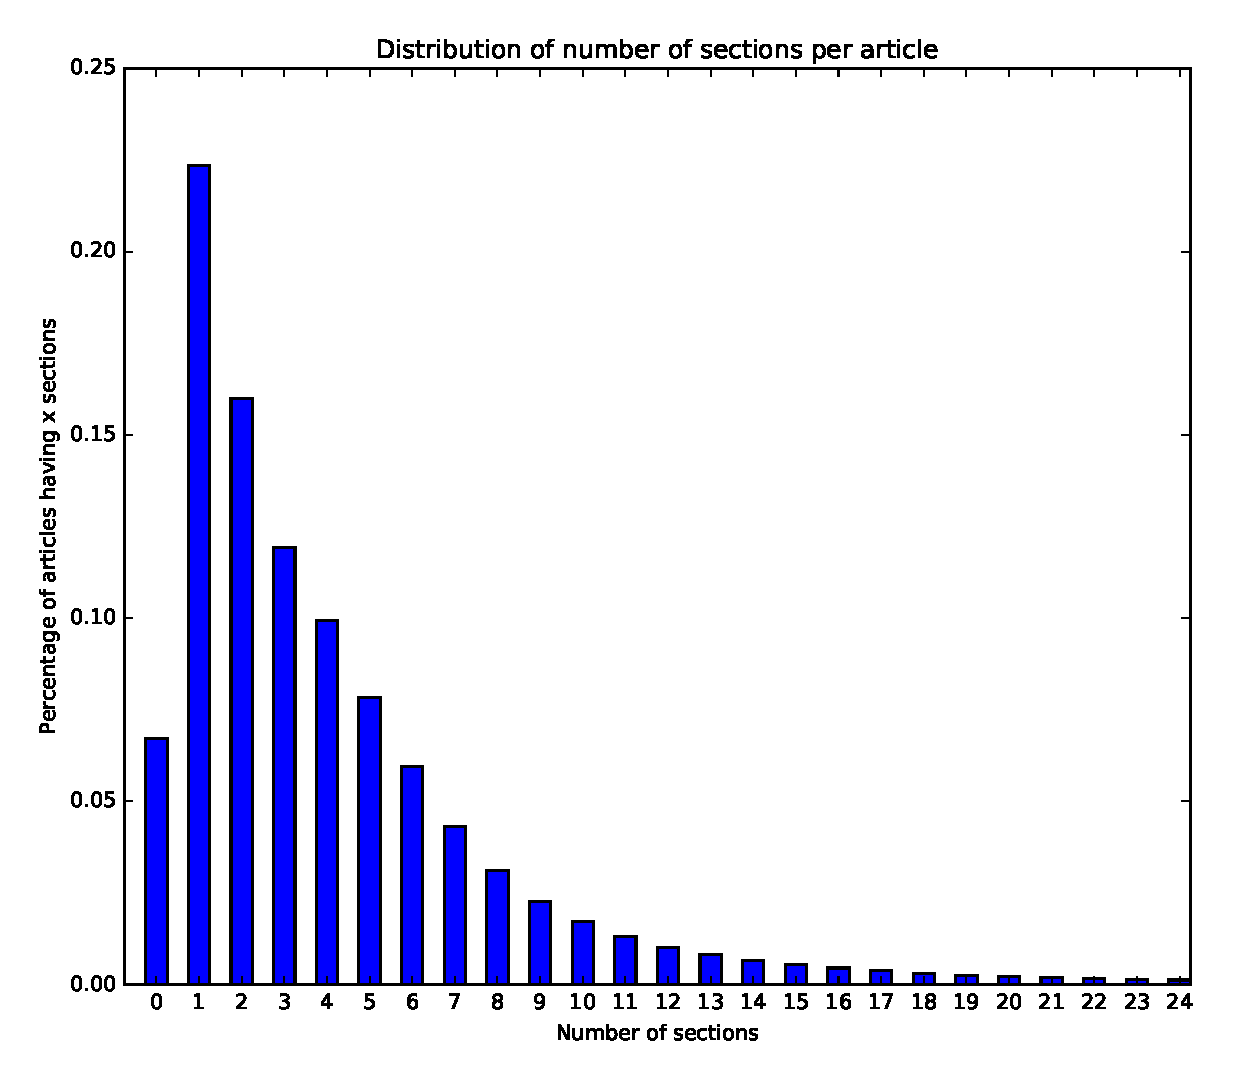
\includegraphics[keepaspectratio=true, width=\textwidth]{assets/section_counts_last_pdf}
\caption{Distribution of the number of sections per article found in the English Wikipedia at the 1st of September, 2015.
Each bar represent how many articles have that number of sections, divided by the total number of articles.}
\label{fig:section_counts_last_pdf}
\end{figure}

Fig.~\ref{fig:section_counts_last_pdf} show the distribution of the number of sections in Wikipedia articles at the time of the snapshot (September 1st, 2015).
The result is somewhat expected from the perspective of a Wikipedia reader: the probability of having $x$ number of sections in an article decreases with the number of sections considered.
However it is interesting to see that the distribution peaks at $x = 1$ number of sections and not at $x = 0$.

To justify this fact a further investigation is required.
However, we hypothesize that articles with less that 2 sections are usually stubs, and that they contains a ``references'' or an ``external links'' sections with the source of information used to create the article.
\todo{is this explanation acceptable?}

\begin{figure}[h]
\centering
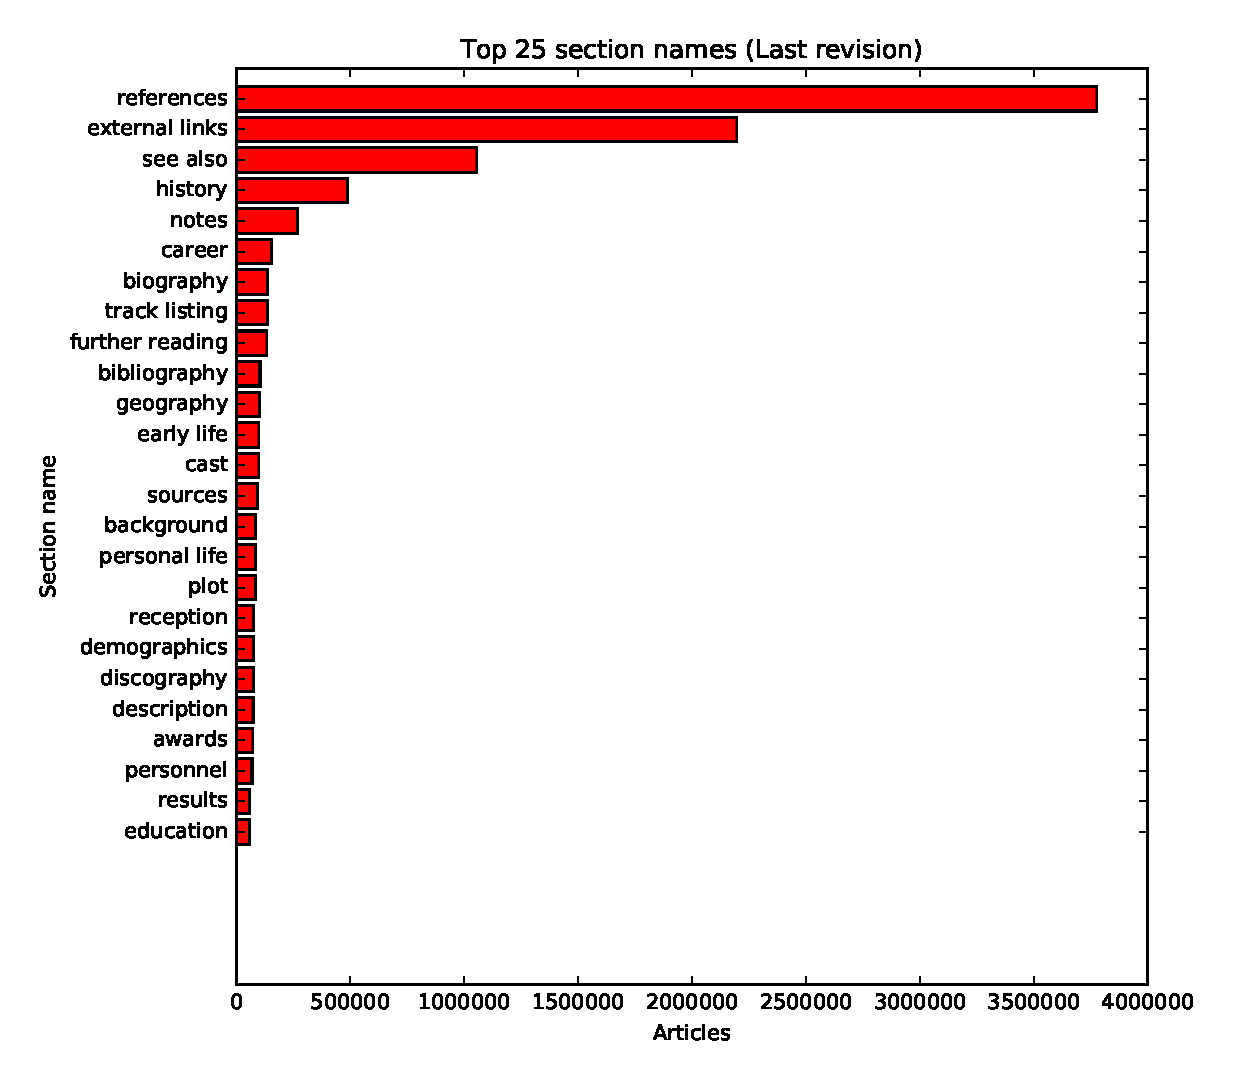
\includegraphics[keepaspectratio=true, width=\textwidth]{assets/section_names_last_top_25}
\caption{Ranking of the top 25 section names found in the English Wikipedia at the 1st of September, 2015.
The value of each bar is the number of articles where that section appears}
\label{fig:section_names_last_top_25}
\end{figure}

It is also interesting to analyze which are the most common section names used.
The result is shown in Fig.~\ref{fig:section_names_last_top_25}.
The most common section used is ``references''.
According to Wikipedia guidelines, this section is intended to contain citations, footnotes and general references.
Therefore it is expected that it appears in the first position of the ranking.
``External links'' usually contains links to the original material described in the article, while in ``see also'' there are usually interlinks to related articles, hence their popularity.

It is also expected to see that topics like ``career'' and ``biography'' appear together, because articles about persons usually include both of them.


\section{Papers in Wikipedia}
This section analyzes the use of papers in wikipedia.

\subsection{Incoming citations distribution}
The distribution of scholarly citations has been studied many times by the scientific community.
The problem is to understand the law that describes the \emph{distribution of citations} of papers, namely the distribution of the number of papers $N(x)$ that have been cited $x$ times.
Redner~\cite{Redner1998} suggested that this distribution has a large-$x$ power law decay $N(x) \sim x^{-\alpha}$ \todo{explain some more of that article}.

\begin{figure}[h]
\centering
\includegraphics[keepaspectratio=true, width=\textwidth]{assets/incoming_cits_loglog}
\caption{Incoming citations distribution of papers appearing in the \emph{mag} datasets and the ones appearing only in English Wikipedia, on a log-log scale.}
\label{fig:incoming_citations_loglog}
\end{figure}

Fig.~\ref{fig:incoming_citations_loglog} compares the distribution of citations of all the papers known to the MAG (circa 120 millions) and the ones whose \ac{DOI} appears in Wikipedia (circa 389 thousands).
The number of incoming citation for a paper is determined using the \ac{MAG} dataset.
Notice that the only identifier available in the \ac{MAG} is the \ac{DOI}, hence only the papers found in Wikipedia which have a \ac{DOI} are considered.
This accounts for the 28\% of the identifiers found.
Furthermore, from this set of papers we removed the ones that appears to be ``non-valid'' in the \ac{MAG} dataset, namely the ones that have more than one \ac{DOI}.
The amount of papers considered at the end is the 17\% of the identifiers found in Wikipedia.

From the graph we can only see that both the distribution follow some kind of power law.
It is more interesting to analyze the \ac{ccdf} of the two series.
In our case, the \ac{ccdf}, or \emph{tail distribution}, expresses the percentage of papers $\bar{F}(x)$ that have more than $x$ citations.

From Fig.~\ref{fig:incoming_citations_ccdf_1000}~and~\ref{fig:incoming_citations_ccdf_100} we can see that papers appearing in Wikipedia tend to have many more incoming citations with respect to a random paper taken from all the available ones.
For instance, the 74\% of papers in Wikipedia have at least 10 incoming citations, while only the 13\% of papers have at least 10 incoming citations.
A plausible explanation is that users tend to insert papers with a higher rank in term of incoming citations, rather than ones with less impact on the scientific community.
\todo{Add graphs comparing various journals}
% see https://en.wikipedia.org/wiki/User:ProteinBoxBot.




\begin{figure}[h]
\centering
\includegraphics[keepaspectratio=true, width=\textwidth]{assets/incoming_cits_ccdf_1000}
\caption{Complementary cumulative distribution function of the first 100 incoming citations of papers appearing in the \emph{mag} datasets and the ones appearing only in English Wikipedia.}
\label{fig:incoming_citations_ccdf_1000}
\end{figure}

\begin{figure}[h]
\centering
\includegraphics[keepaspectratio=true, width=\textwidth]{assets/incoming_cits_ccdf_100}
\caption{Complementary cumulative distribution function of the first 100 incoming citations of papers appearing in the \emph{mag} datasets and the ones appearing only in English Wikipedia.}
\label{fig:incoming_citations_ccdf_100}
\end{figure}

\subsection{Publication date of papers in Wikipedia}
Now we are going to see the publication date distribution of papers appearing in Wikipedia.

\begin{figure}[h]
\centering
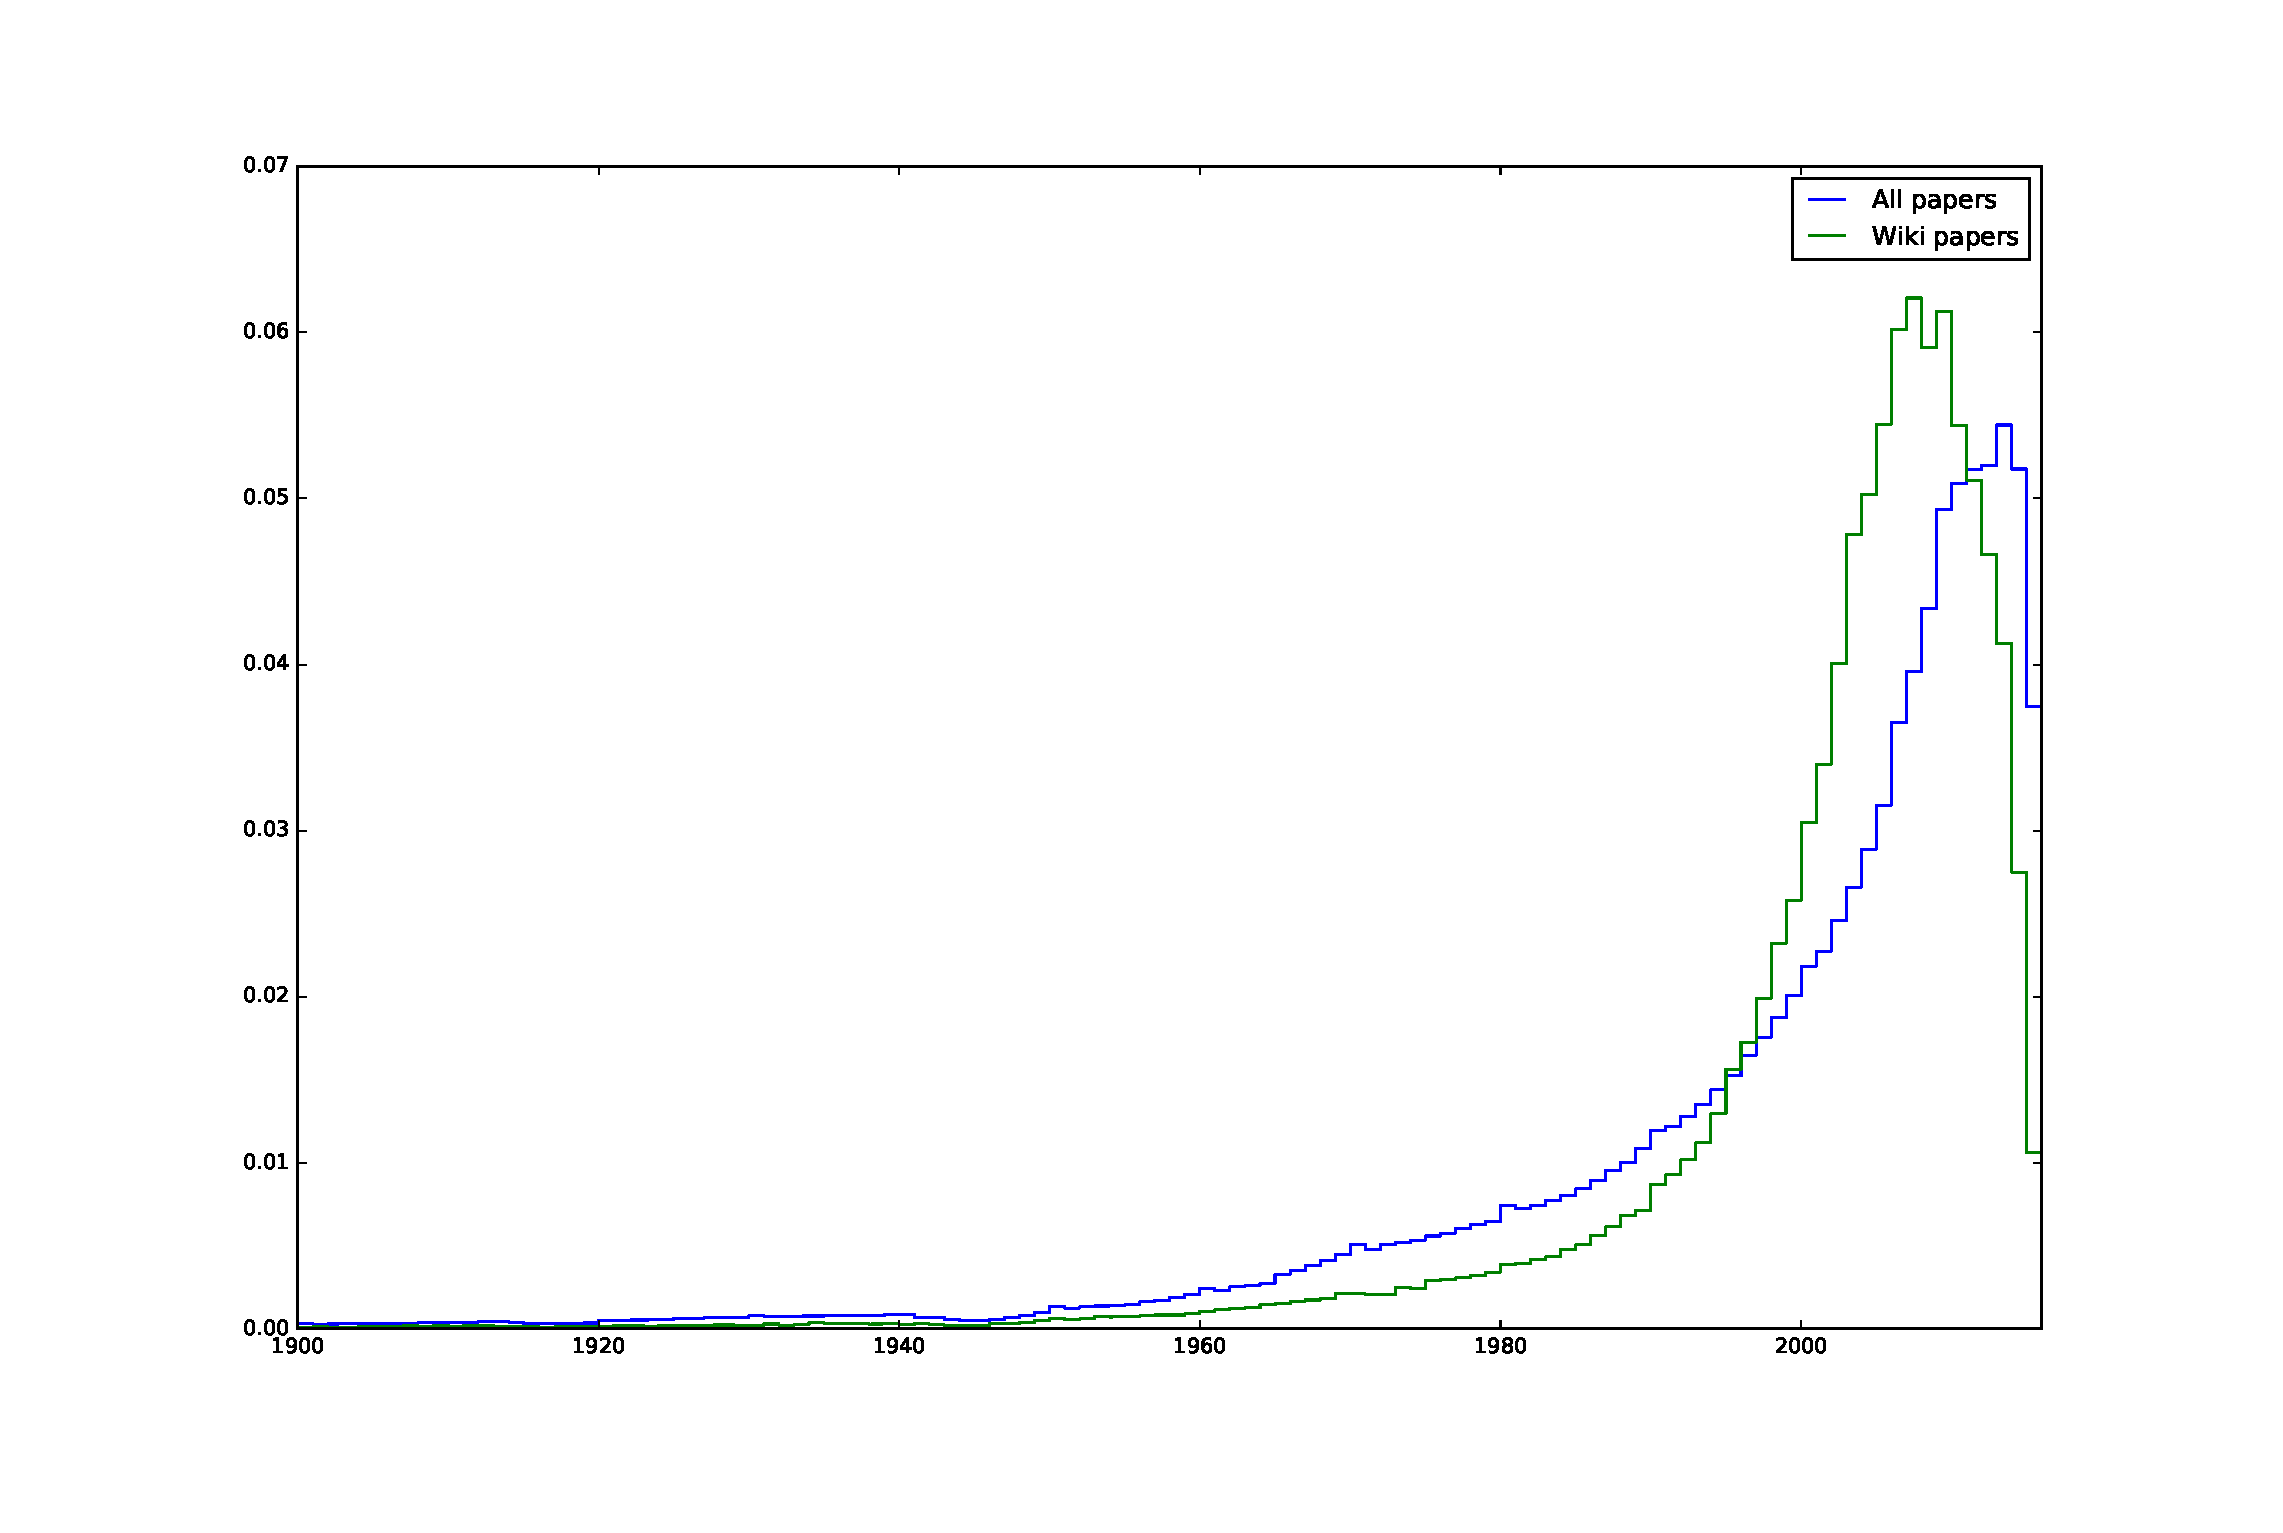
\includegraphics[keepaspectratio=true, width=\textwidth]{assets/publication_date_pdf}
\caption{Publication date distribution of all the known papers form the MAG dataset and the ones found in Wikipedia through the DOIs in the last 60 years, up to the 2014.
}
\label{fig:publication_date_pdf}
\end{figure}

Fig.~\ref{fig:publication_date_pdf} shows exactly this distribution together with a baseline, ``All papers'', representing the distribution of the publication date of all the known papers.
Wikipedia articles tend to cite papers which are released in the last few years.
This is expected because that the number of papers published grows each year and because many works are replicated and extended by other authors and only the newer ones tend to be cited.


% publication growth
In 1961, Price~\cite{Price1961} studied the growth of scientific publications covering the period from about 1650 to 1950.
The data indicated a growth rate of about 5.6\% per year and a doubling time of 13 years.

The study of this matter has then been propose again by many, showing that the growth varies depending on the dataset used and analyzing different period of times.
For instance, Larsen et al.~\cite{Larsen2010} in the 2010 studied the growth using different datasets and limited to the time period between the 1907 and the 2007.
They showed that there are many other factors that determine the growth of publications that should be considered.

We have reproduced the result of Larsen et al.\ using the linear regression method, and we have obtained comparable results: the overall growth rate we have found is about 3,98\% and a doubling time of 17,4 years.
Fig.~\ref{fig:publication_date_regression} compares the actual growth with the one we have derived.

It is interesting to see also which is the distribution of the publication date of papers appearing in Wikipedia, and compare it with the distribution of the publication date of all the paper (Fig.~\ref{fig:publication_date_pdf}).

\begin{figure}[h]
\centering
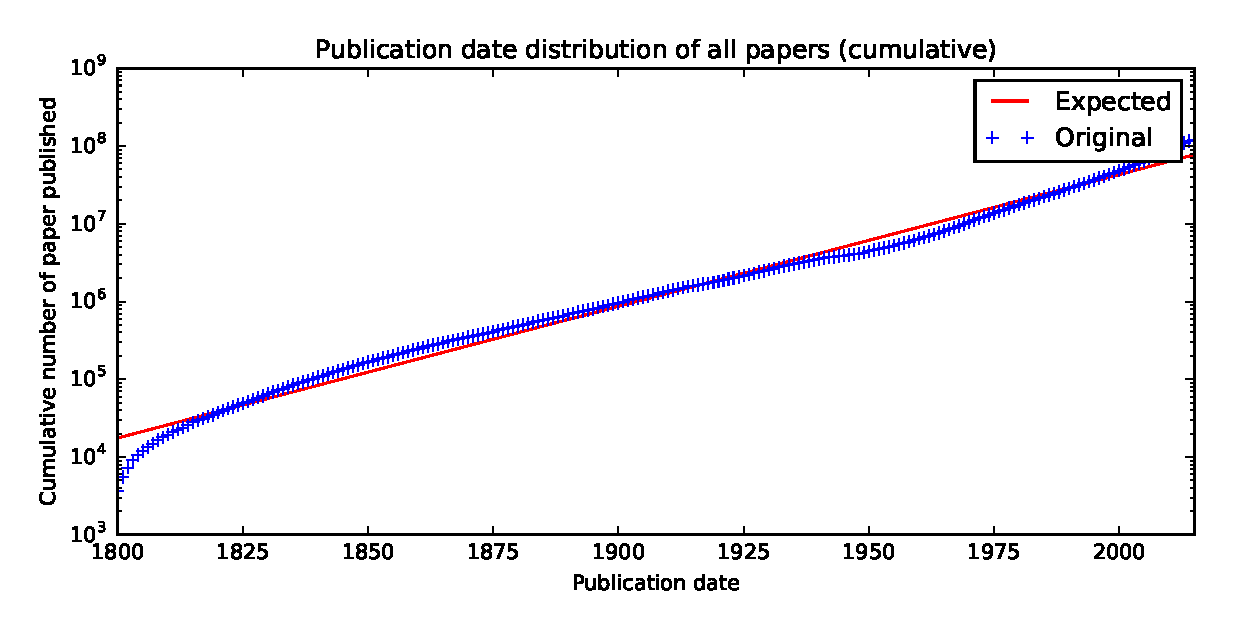
\includegraphics[keepaspectratio=true, width=\textwidth]{assets/publication_date_regression}
\caption{Publication date count for all the papers appearing in the \ac{MAG} dataset and its estimate curve obtained with linear regression}
\label{fig:publication_date_regression}
\end{figure}



\subsection{Age of identifiers at first appearance}
Another interesting information to analyze is the age of the papers when they first appear in Wikipedia.
Fig.~\ref{fig:age_of_papers_at_first_appearance} shows the distribution of the age of papers when they are inserted on Wikipedia for the first time.
In theory there should not be negative values, because this would mean that an identifier appears in Wikipedia before the paper is published.
In practice this happens because the \ac{MAG} dataset is not 100\% accurate, and some publication dates may contain errors.
We have investigated this problem, and it seems to be caused by how Microsoft extracts the publication date of a paper.
It appears that if a paper is published online on a certain date, and it is also released after in a journal, Microsoft consider the date of the journal the publication date.
However, only the 3,12\% of the \acp{DOI} extracted have a negative age, so the effect of the error is arguably quite marginal.

It is interesting to see that many \acp{DOI} are inserted in Wikipedia few days after their publication (Fig.~\ref{fig:age_of_papers_at_first_appearance_zoom}).
We have analyzed some of these cases, and it appears that that some authors insert the identifier of their paper as soon as it has been published.

Finally, to give a scale to this numbers, Fig.~\ref{fig:age_of_papers_at_first_appearance_cdf} measure is the \ac{cdf} of the series, namely what is the percentage $F(x)$ of paper identifiers inserted in Wikipedia at most $x$ days after their publication.
\todo{conclude, somehow}

% Notes:
% Kamil Crater (doi 10.1126/science.1190990) has been added by the author as soon as possible. \url{https://en.wikipedia.org/w/index.php?title=Kamil_Crater&diff=next&oldid=375884625}

\begin{figure}[h]
\centering
\includegraphics[keepaspectratio=true, width=\textwidth]{assets/age_of_papers_at_first_appearance}
\caption{Distribution of the age of papers when their DOI appear for the first time on Wikipedia.}
\label{fig:age_of_papers_at_first_appearance}
\end{figure}

\begin{figure}[h]
\centering
\includegraphics[keepaspectratio=true, width=\textwidth]{assets/age_of_papers_at_first_appearance_-30+30}
\caption{Distribution of the age of papers when their DOI appear for the first time on Wikipedia, showing only ages between $[-30, 30]$ days.}
\label{fig:age_of_papers_at_first_appearance_zoom}
\end{figure}

\begin{figure}[h]
\centering
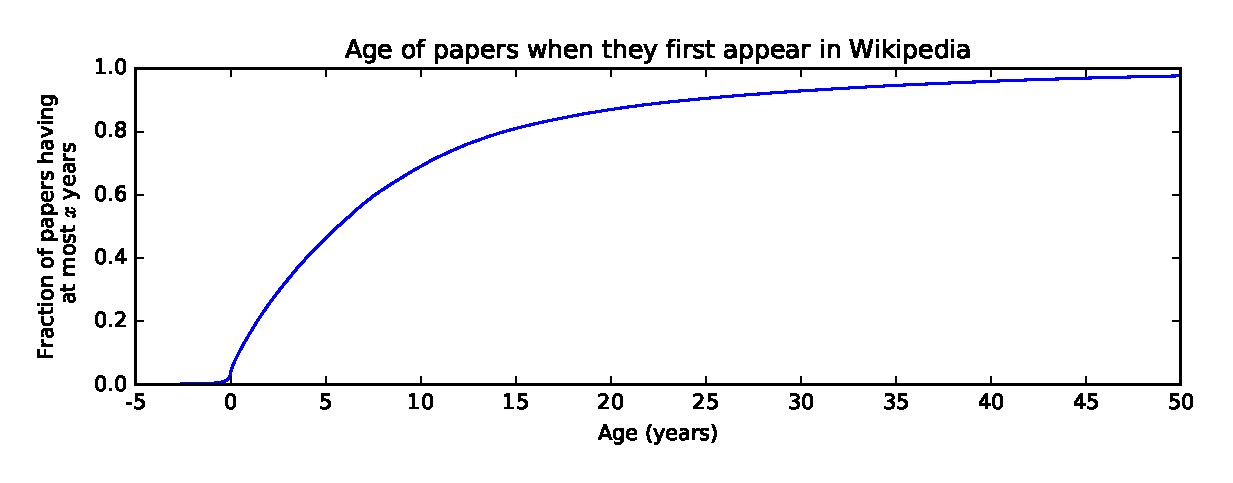
\includegraphics[keepaspectratio=true, width=\textwidth]{assets/age_of_papers_at_first_appearance_cdf}
\caption{todo}
\label{fig:age_of_papers_at_first_appearance_cdf}
\end{figure}


\subsection{Lifetime of irrelevant citations inside an article}
It is interesting to analyze how long academic citations live inside a page.
In particular, the focus of this sections is on publication identifiers which have been inserted in a page and then removed for some reason, most probably because of irrelevance.
The rationale behind this choice is to analyze how long does it take for a Wikipedia contributor to discover and remove an irrelevant identifier appearing in an article.

We define the notion of irrelevance as follows: an identifier is considered \emph{irrelevant} for a Wikipedia article if it appeared on that article in the past but it does no more appear in that page at the time of the snapshot being taken, in our case the 1st of September 2015.

The lifetime of irrelevant identifiers found in different pages is depicted in the left column of Figure~\ref{fig:irrelevant_identifiers_and_dois}, by the meaning of plots displaying the cumulative distribution function.
The ordinate describe how many identifiers in different pages lived at most $x$ time units (e.g.\ years, months or days).
In another way, the graphs show how long did it take for the Wikipedians to remove the irrelevant identifiers from the articles where they appear.
Each series describe the behavior of a certain type of identifier (i.e.\ \ac{ISBN}, \ac{DOI}, \ac{PMID} or \emph{arXiv})
All the curves starts with a steep climb in the first period of time.
Indeed more than the 60\% of irrelevant \ac{ISBN} and \ac{DOI} ``lived'' in articles for less than one year.
Something more worth of notice is that 35\% of \acp{DOI} ``lived'' less than one month, and more than the 20\% less then one day.

However, it may also be the case that many identifiers are removed almost immediately because they are typos made by a contributor while he was editing the page.

We have a way to distinguish \acp{DOI} which are valid (i.e.\ that refer to an existing object) from the ones that are not.
We first search for the DOI in the MAG corpus: if it exists then it is valid, otherwise we query directly the DOI authority using the available APIs\footnote{\url{http://www.doi.org/factsheets/DOIProxy.html}}.


Figure~\ref{fig:irrelevant_identifiers_count} shows the number of \acp{DOI} appearances that are generated by valid and invalid DOIs.
We observe that just the 4\% of them are due to an unrecognized identifier, most probably a typo.
The right column of Figure~\ref{fig:irrelevant_identifiers_and_dois} shows how long DOIs lived inside Wikipedia articles, along with the ones that are not recognized.
We observe, as expected, that the latter do not play a major role in the distribution.
This fact reject the hypothesis that a good part of irrelevant DOIs are removed almost immediately because they are typos made by editors.

Considering the fact that more than the 20\% of irrelevant \acp{ISBN} and \acp{DOI} are removed within the first day, we conclude that the effort made by Wikipedians to remove irrelevant references inside the articles is both remarkable and effective.

\begin{figure}[h]
    \centering
    \begin{subfigure}{.5\textwidth}
        \centering
        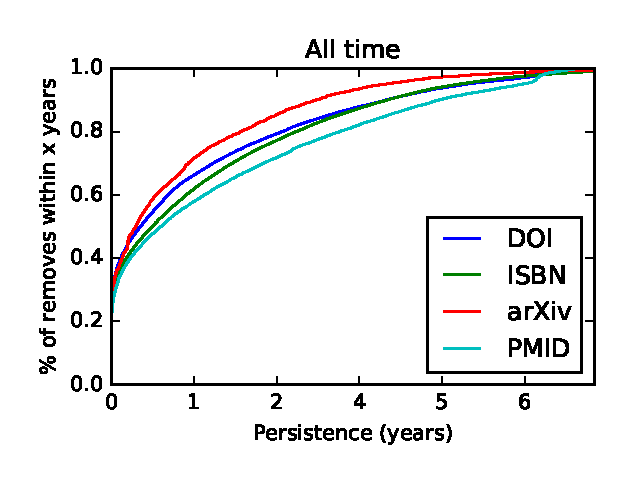
\includegraphics[keepaspectratio=true, width=1\linewidth]{assets/irrelevant_identifiers_persistence_cdf_max}
\label{fig:irrelevant_identifiers_persistence_cdf_max}
    \end{subfigure}%
    \begin{subfigure}{.5\textwidth}
        \centering
        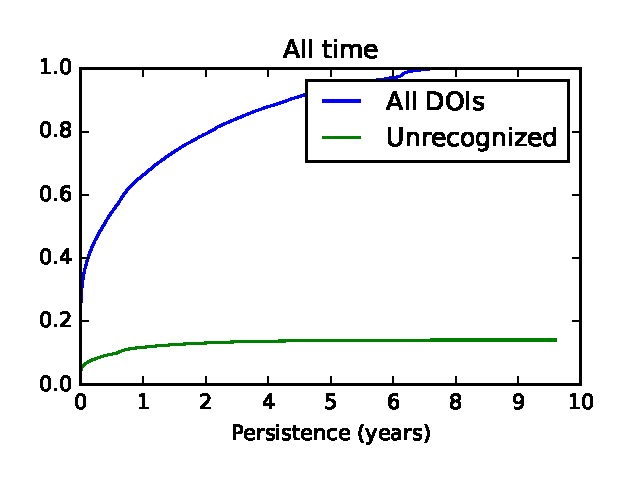
\includegraphics[keepaspectratio=true, width=1\linewidth]{assets/irrelevant_doi_persistence_cdf_max}
\label{fig:irrelevant_doi_persistence_cdf_max}
    \end{subfigure}

    \begin{subfigure}{.5\textwidth}
        \centering
        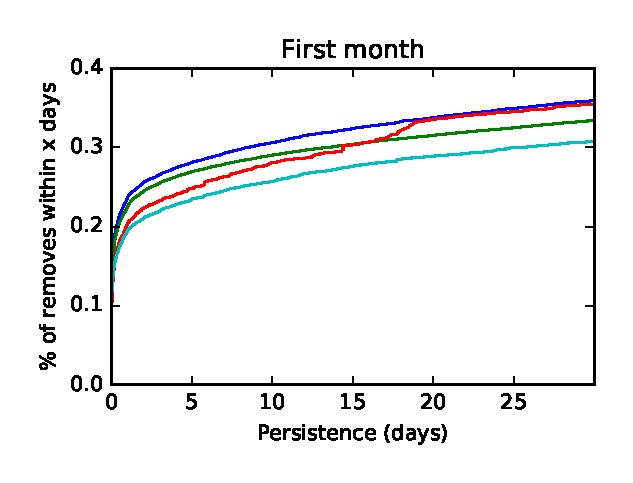
\includegraphics[keepaspectratio=true, width=1\linewidth]{assets/irrelevant_identifiers_persistence_cdf_1month}
\label{fig:irrelevant_identifiers_persistence_cdf_1month}
    \end{subfigure}%
    \begin{subfigure}{.5\textwidth}
        \centering
        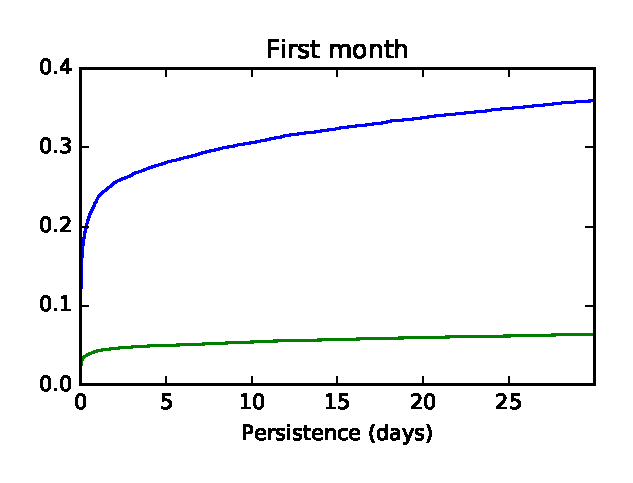
\includegraphics[keepaspectratio=true, width=1\linewidth]{assets/irrelevant_doi_persistence_cdf_1month}
\label{fig:irrelevant_doi_persistence_cdf_1month}
    \end{subfigure}

    \begin{subfigure}{.5\textwidth}
        \centering
        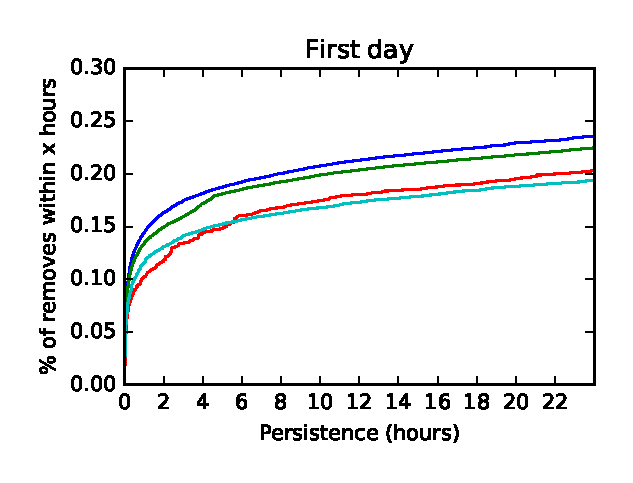
\includegraphics[keepaspectratio=true, width=1\linewidth]{assets/irrelevant_identifiers_persistence_cdf_1day}
\label{fig:irrelevant_identifiers_persistence_cdf_1day}
    \end{subfigure}%
    \begin{subfigure}{.5\textwidth}
        \centering
        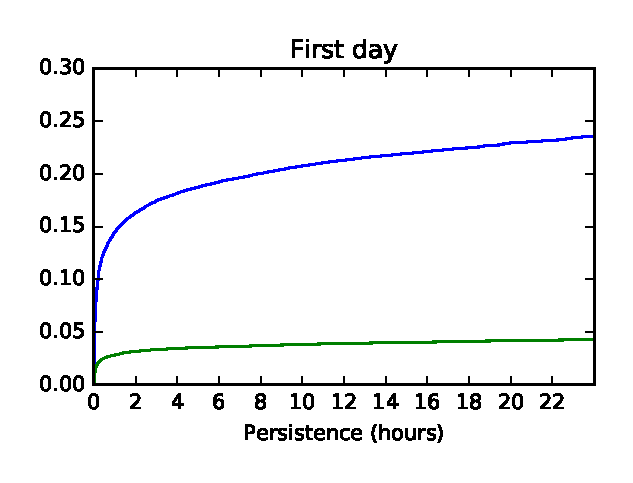
\includegraphics[keepaspectratio=true, width=1\linewidth]{assets/irrelevant_doi_persistence_cdf_1day}
\label{fig:irrelevant_doi_persistence_cdf_1day}
    \end{subfigure}
    \caption{On the left column: distribution of the time required to remove irrelevant identifiers, with a detailed view of the first month and the first day.
    On the right column: distribution of the time required to remove irrelevant DOIs, along with the number of unrecognized DOIs.
    The y-axis describes the ratio of identifier removed in different Wikipedia articles within $x$ time units.}
\label{fig:irrelevant_identifiers_and_dois}
\end{figure}

\begin{figure}[h]
    \centering
    \begin{subfigure}{.5\textwidth}
        \centering
        \includegraphics[keepaspectratio=true, width=\textwidth]{assets/irrelevant_identifiers_count_by_type}
    \end{subfigure}%
    \begin{subfigure}{.5\textwidth}
        \centering
        \includegraphics[keepaspectratio=true, width=\textwidth]{assets/irrelevant_doi_count_by_validity}
    \end{subfigure}
    \caption{On the left side: number of irrelevant identifiers appearances in different Wikipedia articles.
    On the right side: the number of appearances of DOIs not recognized by the authority along with the total number of DOI appearances.}
\label{fig:irrelevant_identifiers_count}
\end{figure}

%A word of caution: we assume that if an identifier has been removed from a page and it is not present in the last revision at the time of the dump, then its appearance in the page is not relevant.



%\subsection{Top cited journals by views}

      \newpage
      % !TEX root = thesis.tex

\chapter{Contributions}
\label{cha:Contributions}

\section{Datasets}
\label{sec:Datasets}

\subsection{Partial dump containing bibliography sections}
\label{sub:contrib_datasets_bibsects}
\todo{Purpose of this dataset? Who can be interested in it?}


\subsection{Page views ordered by project, article}
\label{sub:contrib_datasets_pagecounts}
\todo{Importance of this dataset, maybe cite~\cite{Priedhorsky2007}}

\subsection{History papers in wikipedia, with visits of 2014}


\section{Programs}
\label{sec:Programs}

\subsection{Wikipedia extraction framework}
\label{sub:contrib_programs_framework}
\todo{Decide whether to insert this}


\subsection{Identifiers extraction}
\label{sub:contrib_programs_idextract}
Pull request on Aaron's github repo mwrefs


\subsection{pagecounts-search}
\label{sub:contrib_programs_pagecountssearch}
Programs that search counts by project, article

\subsection{Identifiers in a page visualizer}
Tool to generate the timeline of the identifiers in a wikipedia page.

      \newpage
      % !TEX root = thesis.tex

\chapter{Conclusion and further work}
\label{cha:conclusion}
TODO

      \nocite{*}

    \endgroup


    % bibliografia in formato bibtex
    %
    % aggiunta del capitolo nell'indice
    \addcontentsline{toc}{chapter}{Bibliography}
    % stile con ordinamento alfabetico in funzione degli autori
    \bibliographystyle{plain}
    \bibliography{biblio}
%%%%%%%%%%%%%%%%%%%%%%%%%%%%%%%%%%%%%%%%%%%%%%%%%%%%%%%%%%%%%%%%%%%%%%%%%%
%%%%%%%%%%%%%%%%%%%%%%%%%%%%%%%%%%%%%%%%%%%%%%%%%%%%%%%%%%%%%%%%%%%%%%%%%%
%% Nota
%%%%%%%%%%%%%%%%%%%%%%%%%%%%%%%%%%%%%%%%%%%%%%%%%%%%%%%%%%%%%%%%%%%%%%%%%%
%% Nella bibliografia devono essere riportati tutte le fonti consultate
%% per lo svolgimento della tesi. La bibliografia deve essere redatta
%% in ordine alfabetico sul cognome del primo autore.
%%
%% La forma della citazione bibliografica va inserita secondo la fonte utilizzata:
%%
%% LIBRI
%% Cognome e iniziale del nome autore/autori, la data di edizione, titolo, casa editrice, eventuale numero dell’edizione.
%%
%% ARTICOLI DI RIVISTA
%% Cognome e iniziale del nome autore/autori, titolo articolo, titolo rivista, volume, numero, numero di pagine.
%%
%% ARTICOLI DI CONFERENZA
%% Cognome e iniziale del nome autore/autori (anno), titolo articolo, titolo conferenza, luogo della conferenza (città e paese), date della conferenza, numero di pagine.
%%
%% SITOGRAFIA
%% La sitografia contiene un elenco di indirizzi Web consultati e disposti in ordine alfabetico.
%% E’ necessario:
%%   Copiare la URL (l’indirizzo web) specifica della pagina consultata
%%   Se disponibile, indicare il cognome e nome dell’autore, il titolo ed eventuale sottotitolo del testo
%%   Se disponibile, inserire la data di ultima consultazione della risorsa (gg/mm/aaaa).
%%%%%%%%%%%%%%%%%%%%%%%%%%%%%%%%%%%%%%%%%%%%%%%%%%%%%%%%%%%%%%%%%%%%%%%%%%
%%%%%%%%%%%%%%%%%%%%%%%%%%%%%%%%%%%%%%%%%%%%%%%%%%%%%%%%%%%%%%%%%%%%%%%%%%


    \titleformat{\chapter}
        {\normalfont\Huge\bfseries}{Appendix \thechapter}{1em}{}
    % sezione Allegati - opzionale
    \appendix
    \input{appendices}

\end{document}
